\title{ A Traveling Salesman Solution For The Capitals of All African Nations }
\author{
        Brian Gianforcaro \\
                Department of Computer Science\\
        Rochester Institute of Technology\\
}

\date{\today}

\documentclass[12pt]{article}

\usepackage{graphicx}
\usepackage{multicol}
\usepackage{mdwlist}
\usepackage{amssymb,amsmath}
\usepackage{cite}
\usepackage[bookmarks=false,colorlinks=true,linkcolor={blue},pdfstartview={XYZ null null 1.22}]{hyperref}
\usepackage{url}

\begin{document}
\maketitle

\begin{abstract}
A Traveling Salesman Problem is the task of finding
the shortest round trip path a traveling salesperson can take
to visit each vertex of a given graph.  They are usually
implemented using a genetic algorithm. Our salesperson
happens to be traveling to the capitals of every country in Africa that is a recognized member of the United Nations.
\end{abstract}

\section{The Problem}

\begin{figure}
\begin{center}
\setlength\fboxsep{1.00pt}
\setlength\fboxrule{1.00pt}
\fbox{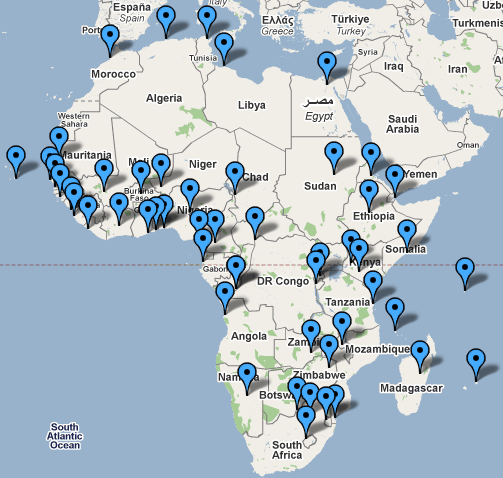
\includegraphics[scale=0.80]{points.png}}
\caption{Capitals of African Nations}
\end{center}
\end{figure}


\begin{multicols}{3}
\tiny\begin{enumerate*}
\item Algeria - Algiers
\item Angola - Luanda
\item Benin - Porto-Novo
\item Botswana - Gaborone
\item Burkina Faso - Ouagadougou
\item Burundi - Bujumbura
\item Cameroon - Yaounde
\item Cape Verde - Praia
\item Central African Republic - Bangui
\item Chad - N'Djamena
\item Comoros - Moroni
\item Congo, Republic of the - Brazzaville
\item Congo, Democratic Republic of the - Kinshasa
\item Cote d'Ivoire - Yamoussoukro
\item Djibouti - Djibouti
\item Egypt - Cairo
\item Equatorial Guinea - Malabo
\item Eritrea - Asmara
\item Ethiopia - Addis Ababa
\item Gabon - Libreville
\item The Gambia - Banjul
\item Ghana - Accra
\item Guinea - Conakry
\item Guinea-Bissau - Bissau
\item Kenya - Nairobi
\item Lesotho - Maseru
\item Liberia - Monrovia
\item Libya - Tripoli
\item Madagascar - Antananarivo
\item Malawi - Lilongwe
\item Mali - Bamako
\item Mauritania - Nouakchott
\item Mauritius - Port Louis
\item Morocco - Rabat
\item Mozambique - Maputo
\item Namibia - Windhoek
\item Niger - Niamey
\item Nigeria - Abuja
\item Rwanda - Kigali
\item Senegal - Dakar
\item Seychelles - Victoria
\item Sierra Leone - Freetown
\item Somalia - Mogadishu
\item South Africa - Pretoria
\item Sudan - Khartoum
\item Swaziland - Mbabane
\item Tanzania - Dar es Salaam
\item Togo - Lome
\item Tunisia - Tunis
\item Uganda - Kampala
\item Zambia - Lusaka
\item Zimbabwe - Harare
\end{enumerate*}
\end{multicols}

\section{Overview}
The remainder of this article is organized as follows.
Section~ gives account of previous work.
Our new and exciting results are described in Section~.
Finally, Section gives the conclusions.

\section{Programs}

The TSP was solved using the Python 2.6 programming language.

I leveraged software written by John Montgomery \cite{cite_key2}

The results were then visualized using Google maps mapping API.

Two methods were used a \bf{hillclimb} and

\section{Solution}

\begin{align}
  yDis = ( lat2 - lat1 ) * Nautical Miles Per Latitude\\
  xDis = ( \cos( lat1 - \frac{\pi}{180} ) + \cos( lat2 - \frac{\pi}{180} ) ) * ( lon2 - lon1 ) * \frac{Nautical Miles Per Longitude}{2}\\
  tDistance = \sqrt{ yDis^{2} + xDis^{2} } * Miles per Nautical Miles\\
\end{align}


\begin{figure}
\begin{center}
\setlength\fboxsep{1.00pt}
\setlength\fboxrule{1.00pt}
\fbox{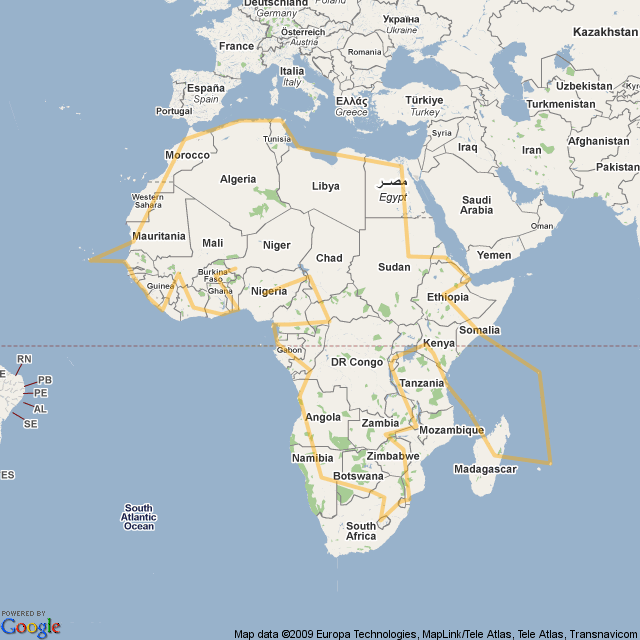
\includegraphics[scale=0.65]{path.png}}
\caption{Final Path Through Africa}
\end{center}
\end{figure}

Final Order:

\begin{multicols}{3}
\tiny\begin{enumerate*}
\item Congo, Republic of the - Brazzaville
\item Congo, Democratic Republic of the - Kinshasa
\item Angola - Luanda
\item Namibia - Windhoek
\item Botswana - Gaborone
\item South Africa - Pretoria
\item Lesotho - Maseru
\item Swaziland - Mbabane
\item Mozambique - Maputo
\item Zimbabwe - Harare
\item Zambia - Lusaka
\item Malawi - Lilongwe
\item Burundi - Bujumbura
\item Rwanda - Kigali
\item Uganda - Kampala
\item Kenya - Nairobi
\item Tanzania - Dar es Salaam
\item Comoros - Moroni
\item Madagascar - Antananarivo
\item Mauritius - Port Louis
\item Seychelles - Victoria
\item Somalia - Mogadishu
\item Ethiopia - Addis Ababa
\item Djibouti - Djibouti
\item Eritrea - Asmara
\item Sudan - Khartoum
\item Egypt - Cairo
\item Libya - Tripoli
\item Tunisia - Tunis
\item Algeria - Algiers
\item Morocco - Rabat
\item Mauritania - Nouakchott
\item Cape Verde - Praia
\item Senegal - Dakar
\item The Gambia - Banjul
\item Guinea-Bissau - Bissau
\item Guinea - Conakry
\item Sierra Leone - Freetown
\item Liberia - Monrovia
\item Cote d'Ivoire - Yamoussoukro
\item Mali - Bamako
\item Burkina Faso - Ouagadougou
\item Niger - Niamey
\item Ghana - Accra
\item Togo - Lome
\item Benin - Porto-Novo
\item Nigeria - Abuja
\item Chad - N'Djamena
\item Central African Republic - Bangui
\item Cameroon - Yaounde
\item Equatorial Guinea - Malabo
\item Gabon - Libreville
\end{enumerate*}
\end{multicols}

In this section we describe the results.

\section{Runtime}
We worked hard, and achieved very little.

\section{Analysis}

\begin{thebibliography}{99}
\bibitem{cite_key1} Montgomery, John {\it Tackling The Travelling Salesman Problem}{\href{http://www.psychicorigami.com/category/tsp/}{ http://www.psychicorigami.com/category/tsp/} }, {\bf 2007}
\bibitem{cite_key2} Mead, C. A.; Truhlar, D. G. {\it J. Chem. Phys.} {\bf 1983}, {\it 78}, 6344.
\end{thebibliography}
\end{document}
